%===================================================
%================== DOCUMENT CLASS
%===================================================
\documentclass[runningheads,11pt,a4paper,english,llncs]{Misc/llncs}

%===================================================
%================== PACKAGES
%===================================================
%------------------------------------------------------------------------
% TeX and LaTeX macros
%------------------------------------------------------------------------
%
% In math formulas we use italic instead of mathitalic
%
\makeatletter
% ~ gives a \; space in math mode
\def~{\ifmmode\;\else\penalty\@M\ \fi}
%  Italic in mathematical formulas
\def\@setmcodes#1#2#3{{\count0=#1 \count1=#3
  \loop \global\mathcode\count0=\count1 \ifnum \count0<#2
  \advance\count0 by1 \advance\count1 by1 \repeat}}
\DeclareSymbolFont{italic}{OT1}{\rmdefault}{m}{it}
\let\mathit\undefined
\DeclareSymbolFontAlphabet{\mathit}{italic}
\edef\@tempa{\hexnumber@\symitalic}
\@setmcodes{`A}{`Z}{"7\@tempa41}
\@setmcodes{`a}{`z}{"7\@tempa61}
\makeatother
%
% \begin{asm} ... \end{asm}
%
\newdimen\asmindent     
\asmindent=\parindent
\newcount\asmi
\def\inc{\global\advance\asmi by 1}
\def\dec{\global\advance\asmi by-1}
\def\nl{{}$\par\hangindent\asmi em
  \noindent\kern\asmi em\ignorespaces$} 
\def\asmskip{{}$\par\smallskip\hangindent\asmi em
  \noindent\kern\asmi em\ignorespaces$}

%%%%%%%%%%%%%%%%%%%%%%%%%%%
\def\asm{\global\asmi=0 
 \def\+{\inc\nl}
 \def\-{\dec\nl}
 \def\\{\nl}
 %%% Added by Paolo 2018-06-25:
 \setlength{\parskip}{0pt}
 %%%
 \begin{trivlist}\item[]\leftskip=\asmindent\relax$}
%%%%%%%%%%%%%%%%%%%%%%%%%%%

\def\endasm{$\end{trivlist}}
%\mathindent=\asmindent
%
% \begin{asmarray}
%    f(s_1) & := t_1 \\
%    f(s_2) & := t_2 
% \end{asmarray}
%
\def\asmarray{\begin{array}[t]{@{}l@{\;}l@{\;}l@{}}}
\def\endasmarray{\end{array}}
%
%
%
\def\asmcomment#1{\quad\hbox{// #1}}
%
%  \begin{subasm} ... \end{subasm}
%
\newcount\asmii
\def\subasm{\vtop\bgroup\asmii=0\normalbaselines
 \def\nl##1{$\egroup\advance\asmii by##1\relax\hbox\bgroup\hskip\asmii em$}
 \def\\{\nl{0}}
 \def\+{\nl{1}}
 \def\-{\nl{-1}}
 \hbox\bgroup\hskip\asmii em$}
\def\endsubasm{$\egroup\egroup}
%
% Keywords in ASM code
%
\def\ASM#1{\hbox{\sc#1}}        % rule names and macros
\def\ASMIND#1{\ASM{#1}\index{#1@{\sc#1}}}
\def\AWAIT   {\mathrel{\mathbf{await}}}
\def\AND     {\mathrel{\mathbf{and}}}
\def\CASE    {\mathrel{\mathbf{case}}}
\def\CHOOSE  {\mathrel{\mathbf{choose}}}
\def\CREATE  {\mathrel{\mathbf{create}}}
\def\NEW  {\mathrel{\mathbf{new}}}
\def\DO      {\mathrel{\mathbf{do}}}
\def\ELSE    {\mathrel{\mathbf{else}}}
\def\ELSEIF  {\mathrel{\mathbf{elseif}}}
\def\FORALL  {\mathrel{\mathbf{forall}}}
\def\FORSOME  {\mathrel{\mathbf{forsome}}}
\def\FOREACH  {\mathrel{\mathbf{foreach}}}
\def\THEREISNO  {\mathrel{\mathbf{thereisno}}}
\def\FROM  {\mathrel{\mathbf{from\colon}}}
\def\FOR  {\mathrel{\mathbf{for\colon}}}
\def\TO  {\mathrel{\mathbf{to\colon}}}
\def\IF      {\mathrel{\mathbf{if}}}
\def\IFF      {\mathrel{\mathbf{iff}}}
\def\IMPORT  {\mathrel{\mathbf{import}}}
\def\IN      {\mathrel{\mathbf{in}}}
\def\LET     {\mathrel{\mathbf{let}}}
\def\SELF    {\mathrel{\mathbf{self}}}
\def\MATCH    {\mathrel{\textbf{match}}}
\def\NOT     {\mathrel{\mathbf{not}}}
\def\OF      {\mathrel{\mathbf{of}}}
\def\OR      {\mathrel{\mathbf{or}}}
\def\PAR     {\mathrel{\mathbf{par}}}
\def\SEQ     {\mathrel{\mathbf{seq}}}
\def\SKIP    {\mathrel{\mathbf{skip}}}
\def\THEN    {\mathrel{\mathbf{then}}}
\def\WHERE   {\mathrel{\mathbf{where}}}
\def\WHILE   {\mathrel{\mathbf{while}}}
\def\UNDEF   {\mathrel{\mathbf{undef}}}
\def\UNTIL   {\mathrel{\mathbf{until}}}
\def\WHEN   {\mathrel{\mathbf{when}}}
\def\WITH    {\mathrel{\mathbf{with}}}
\def\STEP    {\mathrel{\mathbf{step}}}
\def\STEPWISE    {\mathrel{\mathbf{stepwise}}}
\def\SEQ    {\mathrel{\mathbf{seq}}}
\def\RESULT  {\mathrel{\mathbf{result}}}
\def\CALL  {\mathrel{\mathbf{Call}}}
\def\LOCAL    {\mathrel{\mathbf{local}}}
\def\ADDGUARD {\mathrel{\mathbf{addGuard}}}
\def\ADDUPD   {\mathrel{\mathbf{addUpd}}}
\def\ADDRULE  {\mathrel{\mathbf{addRule}}}
\def\MINUSRULE  {\mathrel{\mathbf{minusRule}}}
%\def\TO      {\mathrel{\mathbf{to}}}
%
% Including figures
%
\def\includefig#1#2{\centering\medskip
  \includegraphics[scale=#1]{fig/#2}
  \medskip}
%
% References to paragraphs in the ECMA standard for C#
%
\def\ecma#1{\cite[\S#1]{ecma334}}
%
%  Environments for definitions and theorems
%
%\theorembodyfont{\rm}
%\newtheorem{definition}[subsection]{Definition}
%\newtheorem{lemma}[subsection]{Lemma}
%\newtheorem{theorem}[subsection]{Theorem}
%\newtheorem{proposition}[subsection]{Proposition}
%\newtheorem{corollary}[subsection]{Corollary}
%\newtheorem{example}[subsection]{Example}
%\newtheorem{remark}[subsection]{Remark}
%\newtheorem{constraint}[subsection]{Constraint}
\def\proof{\trivlist\item[]{\bf Proof.}}
\def\endproof{$\Box$\endtrivlist}
%
% enumerate and itemize (smaller skips) from "latex.ltx"
%
\makeatletter
\def\enumerate{%
  \ifnum \@enumdepth >\thr@@\@toodeep\else
    \advance\@enumdepth\@ne
    \edef\@enumctr{enum\romannumeral\the\@enumdepth}%
      \expandafter
      \list
        \csname label\@enumctr\endcsname
        {\usecounter\@enumctr\def\makelabel##1{\hss\llap{##1}}
         \itemsep 0pt\parskip 0pt\parsep 0pt\topsep\smallskipamount}%
  \fi}
\def\itemize{%
  \ifnum \@itemdepth >\thr@@\@toodeep\else
    \advance\@itemdepth\@ne
    \edef\@itemitem{labelitem\romannumeral\the\@itemdepth}%
    \expandafter
    \list
      \csname\@itemitem\endcsname
      {\def\makelabel##1{\hss\llap{##1}}
       \itemsep 0pt\parskip 0pt\parsep 0pt\topsep\smallskipamount}%
  \fi}
\makeatother
%
% items in itemize
%
\def\bull{\vrule height .9ex width .8ex depth -.1ex}
\def\labelitemi{\bull}
%
%
%
\def\cs#1{C\#$_{\mathcal{#1}}$}
\def\lang#1{L$_{\mathcal{#1}}$}
%
% Positions
%
\def\pos#1{{}^{#1}}
\def\termPos{\blacktriangleright}
\def\cursor{\pos{\termPos}}
%
%
%
\def\sup{\hbox{sup}}
\def\c#1{\texttt{#1}}           % code
\def\N#1{\textit{#1}}           % non terminal symbols
\def\T#1{\hbox{`\texttt{#1}'}}  % terminal symbols
\def\A#1{\hbox{\sc#1}}          % ASM rules
\def\D#1{#1}                    % dynamic functions
\def\U#1{#1}                    % universes
\def\C#1{#1}                    % constructors
\def\rdef{\equiv}
\def\lbr{\c{\char`\{}}
\def\rbr{\c{\char`\}}}
\def\mb{\hbox{::}}
\def\map#1#2{\textbf{Map from}~#1~\textbf{to}~#2}
\def\cat{\cdot}
\def\adots{\mathinner{\ldotp\ldotp}}
%
%
% macros.tex ends here

\usepackage{bera}% optional: just to have a nice mono-spaced font
\usepackage{listings}
\usepackage{xcolor}

\colorlet{punct}{red!60!black}
\definecolor{background}{HTML}{FFFFFF}
\definecolor{delim}{RGB}{20,105,176}
\colorlet{numb}{magenta!60!black}

\lstdefinelanguage{json}{
    basicstyle=\normalfont\ttfamily,
    commentstyle=\color{eclipseStrings}, % style of comment
    stringstyle=\color{eclipseKeywords}, % style of strings
    numbers=left,
    numberstyle=\scriptsize,
    stepnumber=1,
    numbersep=8pt,
    showstringspaces=false,
    breaklines=true,
    frame=lines,
	string=[s]{"}{"},
    comment=[l]{:\ "},
    morecomment=[l]{:"},
}
\usepackage{bera}% optional: just to have a nice mono-spaced font
\usepackage{listings}
\usepackage{xcolor}
\definecolor{eclipseStrings}{RGB}{42,0.0,255}
\definecolor{eclipseComment}{RGB}{63,127,95}
\definecolor{eclipseKeywords}{RGB}{127,0,85}

\lstdefinelanguage{bsl}{
    % list of keywords
  	morekeywords={
		universe, controlled, location,
    	if, then, endif,
	    while,    	
    	send,
    	or, and, to, in, do, with,
		CoreASIM,
		policy,
		use,
		init,
		rule,
		scheduling, schedule,
    	subject,
    	forall,
    	choose,
		derived,
    	skip, undef,
    	case, endcase, 
    	seq, endseq, par, endpar, block, endblock, next,
    	createASIM, destroyASIM, initializedBy, withProgram, andPolicy,
  	},
  	sensitive=true, % keywords are not case-sensitive
  	morecomment=[l]{//}, % l is for line comment
  	morecomment=[s]{/*}{*/}, % s is for start and end delimiter
  	morestring=[b]" % defines that strings are enclosed in double quotes
}

% Set Language
\lstset{
  language={bsl},
  basicstyle=\normalfont\ttfamily, % Global Code Style
  captionpos=b, % Position of the Caption (t for top, b for bottom)
  extendedchars=true, % Allows 256 instead of 128 ASCII characters
  tabsize=2, % number of spaces indented when discovering a tab 
  columns=fixed, % make all characters equal width
  keepspaces=true, % does not ignore spaces to fit width, convert tabs to spaces
  showstringspaces=false, % lets spaces in strings appear as real spaces
  breaklines=true, % wrap lines if they don't fit
  commentstyle=\color{eclipseComment}, % style of comments
  keywordstyle=\color{eclipseKeywords}, % style of keywords
  stringstyle=\color{eclipseStrings}, % style of strings
}

\lstdefinelanguage{bsl_lst}{
    % list of keywords
  	morekeywords={
		universe, controlled, location,
    	if, then, endif,
	    while,    	
    	send,
    	or, and, to, in, do, with,
		CoreASIM,
		policy,
		use,
		init,
		rule,
		scheduling, schedule,
    	subject,
    	forall,
    	choose,
		derived,
    	skip, undef,
    	case, endcase, of,
    	seq, endseq, par, endpar, block, endblock, next,
    	createASIM, destroyASIM, initializedBy, withProgram, andPolicy,
  	},
  	sensitive=true, % keywords are not case-sensitive
  	morecomment=[l]{//}, % l is for line comment
  	morecomment=[s]{/*}{*/}, % s is for start and end delimiter
  	morestring=[b]", % defines that strings are enclosed in double quotes
  	frame=lines,
  	basicstyle=\normalfont\ttfamily, % Global Code Style
	basicstyle=\normalfont\ttfamily, % Global Code Style
    captionpos=b, % Position of the Caption (t for top, b for bottom)
    extendedchars=true, % Allows 256 instead of 128 ASCII characters
    tabsize=2, % number of spaces indented when discovering a tab 
    columns=fixed, % make all characters equal width
    keepspaces=true, % does not ignore spaces to fit width, convert tabs to spaces
    showstringspaces=false, % lets spaces in strings appear as real spaces
    breaklines=true, % wrap lines if they don't fit
    numbers=left, % show line numbers at the left
    numberstyle=\tiny\ttfamily, % style of the line numbers
    commentstyle=\color{eclipseComment}, % style of comments
    keywordstyle=\color{eclipseKeywords}, % style of keywords
    stringstyle=\color{eclipseStrings}, % style of strings
}
\usepackage{etex}
\reserveinserts{28}
\newcommand{\todo}[1]{
 \noindent{\newline \color{red}
 \framebox[\textwidth][t]{%
  \parbox[t]{0.9\textwidth}{\textcolor{red}{TODO: #1}}                                                                                     
}}}
\usepackage{listings}
\lstset{
  basicstyle=\ttfamily,
  columns=fullflexible,
  breaklines=true,
  postbreak=\mbox{\textcolor{red}{$\hookrightarrow$}\space},
}
\usepackage{graphicx}
\usepackage{acronym}
\usepackage{ifthen}
\usepackage{substr}
\usepackage{color}
\usepackage{fixltx2e}
\usepackage[left=2cm, top=2cm, right=2cm, bottom=2cm]{geometry}
%\usepackage{subfigure}
\usepackage{array}  
\usepackage[figuresright]{rotating}          
\usepackage{url}
\usepackage{tikz}
\usetikzlibrary{trees}
%\usepackage{enumerate}
\usepackage[shortlabels]{enumitem}
\usepackage{epsfig}
\usepackage{colordvi}
\usepackage{makeidx}
\usepackage{index}
\usepackage[absolute]{textpos}
\setlength{\TPHorizModule}{\paperwidth}
\setlength{\TPVertModule}{\TPHorizModule}
\textblockorigin{-6mm}{0mm}
\usepackage[%
      breaklinks=true,%
      colorlinks=true,%           no frame around URL
      urlcolor=LINK_COLOR,%            no colors
      menucolor=LINK_COLOR,%           no colors
      linkcolor=LINK_COLOR,%           no colors
      pagecolor=LINK_COLOR,%           no colors
      bookmarks=true,%            tree-like TOC
      bookmarksopen=false,%       expanded when starting
      hyperfootnotes=true,%       no referencing of footnotes, does not compile
      citecolor=CITE_COLOR,%           black cites
      filecolor=black,%           black files%
      hyperindex=true,%
      hyperfigures=true%
]{hyperref}
\usepackage{bookmark}
\usepackage{booktabs}
\usepackage{dsfont}
\usepackage{wallpaper}
\usepackage{mathtools,cancel}
\usepackage{soul}
\usepackage{float}
\usepackage{setspace}
%\usepackage{morefloats}
%\usepackage{mdwlist}
\usepackage{amsmath,amssymb,amscd,diagrams,bm,amsfonts}
\let\proof\relax
\let\endproof\relax
\usepackage{amsthm}
\usepackage{tabularx, graphics, longtable, multirow, makecell}

%%%%%%% Added by Paolo 2018-03:
\usepackage[justification=centering]{caption}
\usepackage{eurosym}
%%%%%%%%%%%%%%%%%%%%%%

%\usepackage[title]{appendix}


%TIKZ
\usepackage{tikz}
\usepackage{tikz-cd}
\usetikzlibrary{trees,snakes}
\usetikzlibrary{arrows,automata}
\usetikzlibrary{matrix,arrows,positioning}
\usetikzlibrary{mindmap,backgrounds}
\usetikzlibrary{shapes}
\usepackage{verbatim} %for comment out some texts

%%%%%%%%%%%%%%%%%%%%%%%%%%%%%%%
%%%%%%%%%%%%%%%%%%%%% Egon's commands:
\usepackage{latexsym}
\ifx\pdfoutput\undefined
  \message{We are running LaTeX.} 
%PD  \usepackage[dvips]{graphicx}
%PD  \DeclareGraphicsExtensions{.eps}
%PD  \usepackage[hypertex,bookmarks=false]{hyperref}
\else
  \message{We are running PDFLaTeX.}
%PD  \usepackage[pdftex]{color}
%PD  \usepackage[pdftex]{graphicx}
%PD\DeclareGraphicsExtensions{.jpg,.pdf}
%PD  \DeclareGraphicsExtensions{.pdf}
%PD  \usepackage[pdftex,bookmarks=false]{hyperref}
%PD  \hypersetup{colorlinks={true},
%PD            linkcolor={blue},
%PD            citecolor={blue},
%PD            urlcolor={blue},
%PD            plainpages={false}
%PD  }
\fi
%%%%%%%%%%%%%%%%%%%%%%%%%%%%%%%
%%%%%%%%%%%%%%%%%%%%%%%%%%%%%%%

%===================================================
%================== THEOREMS
%===================================================
\theoremstyle{plain}
\newtheorem{thm}{Theorem}
\newtheorem{cor}[thm]{Corollary}
\newtheorem{lem}[thm]{Lemma}
\newtheorem{prop}[thm]{Proposition}
\newtheorem{defin}[thm]{Definition}
\newtheorem{rmrk}[thm]{Remark}

\allowdisplaybreaks


%===================================================
%================== COLOURS
%==================================================

\definecolor{green}{rgb}{0,0.6,0} 
\definecolor{gray}{rgb}{0.6,0.6,0.6} 
\definecolor{red}{rgb}{1,0,0} 
\definecolor{blue}{rgb}{0,0,1} 
\definecolor{purple}{rgb}{0.5,0,0.5} 
\definecolor{yellow}{rgb}{0.25,0.25,0} 
\definecolor{turquoise}{rgb}{0,0.5,0.5}
\definecolor{brown}{rgb}{0.6,0.2,0.1}

\definecolor{LINK_COLOR}{rgb}{0,0,0.7}
\definecolor{CITE_COLOR}{rgb}{0,0.5,0}
\definecolor{lightblue}{rgb}{0,0,1}
\definecolor{light-gray}{gray}{0.95}
\def\red#1{\textcolor[rgb]{1.0,0.0,0.0}{#1}}
\def\green#1{\textcolor[rgb]{0.0,0.8,0.1}{#1}}
\def\blue#1{\textcolor[rgb]{0.0,0.0,1.0}{#1}}

%===================================================
%================== LAYOUT
%===================================================
\parindent=0cm
%\setlength{\parskip}{1.0\baselineskip plus 0.5ex minus 0.2ex}
\abovecaptionskip=0cm
\hyphenpenalty=5000
\tolerance=1000 
\floatsep=1in
\allowdisplaybreaks
\def \constzeroindent {0cm}
\def \constfirstindent {0.5cm}
\def \constsecondindent {1cm}
\newenvironment{mycustomindent}[1]
{\setlength{\parindent}{#1}}
{\setlength{\parindent}{\constzeroindent}}
\newcommand{
	\firstindent}[1]{
	\begin{mycustomindent}{\constfirstindent}
	\begin{tabular}{@{}p{12cm}@{}}
	#1 \\
	\end{tabular}
	\end{mycustomindent}
}
\newcommand{
	\secondindent}[1]{
	\begin{mycustomindent}{\constsecondindent}
	\begin{tabular}{@{}p{12cm}@{}}
	#1 \\
	\end{tabular}
	\end{mycustomindent}
}
\newenvironment{packed_item1}{
\begin{itemize}[topsep=0pt, partopsep=0pt]
  \setlength{\itemsep}{5pt}
  \setlength{\parskip}{0pt}
  \setlength{\parsep}{0pt}
}{\end{itemize}}
\newenvironment{packed_item2}{
\begin{itemize}[topsep=0pt, partopsep=0pt]
  \setlength{\itemsep}{0pt}
  \setlength{\parskip}{0pt}
  \setlength{\parsep}{0pt}
}{\end{itemize}}
\newenvironment{packed_enumerate}{
\begin{enumerate}[topsep=0pt, partopsep=0pt]
  \setlength{\itemsep}{5pt}
  \setlength{\parskip}{0pt}
  \setlength{\parsep}{0pt}
}{\end{enumerate}}
% The following commands are to get rid of the extra space around section and subsection titles:
% Save the class definition of \subparagraph:
\let\llncssubparagraph\subparagraph
% Provide a definition to \subparagraph to keep titlesec happy:
\let\subparagraph\paragraph
\usepackage[compact]{titlesec}
\usepackage{dblfloatfix,caption,subcaption}
\titlespacing{\section}{0pt}{12pt}{*0}
\titlespacing{\subsection}{0pt}{6pt}{0pt}
\titlespacing{\subsubsection}{0pt}{6pt}{0pt}
% Force section numbering to follow chapter numbering:
\usepackage{chngcntr}
\counterwithin{section}{chapter}
\counterwithin{figure}{chapter}
%\counterwithin{theorem}{chapter}
%\counterwithin{lemma}{chapter}
%\counterwithin{definition}{chapter}
%%%%%%%%%%%%%%%%%%%%%%%%%%%%
% Allow line breaks in long list of citations that would extend into the margin:
\usepackage{breakcites}
%%%%%%%%%%%%%%%%%%%%%%%%%%%%%%%%%%%%%%

\usepackage{pdfpages}
\pagestyle{headings}

\renewcommand{\rightmark}{INTERLACE Project (Grant no.~754494)}
\renewcommand{\leftmark}{D3.1}
\setcounter{tocdepth}{2}

\usepackage{tocloft}
\setlength\cftparskip{0pt}
\setlength\cftbeforechapskip{12pt}

%\renewcommand{\cfttoctitlefont}{\normalfont\MakeUppercase}

\usepackage{abstract}
\renewcommand{\abstractnamefont}{\large \bfseries}
%\setlength{\abstitleskip}{-\absparindent}
\renewcommand{\abstractname}{Abstract}

\setlength{\parskip}{12pt}

\begin{document}
%===================================================
%================== TITLE
%===================================================

\thispagestyle{empty}
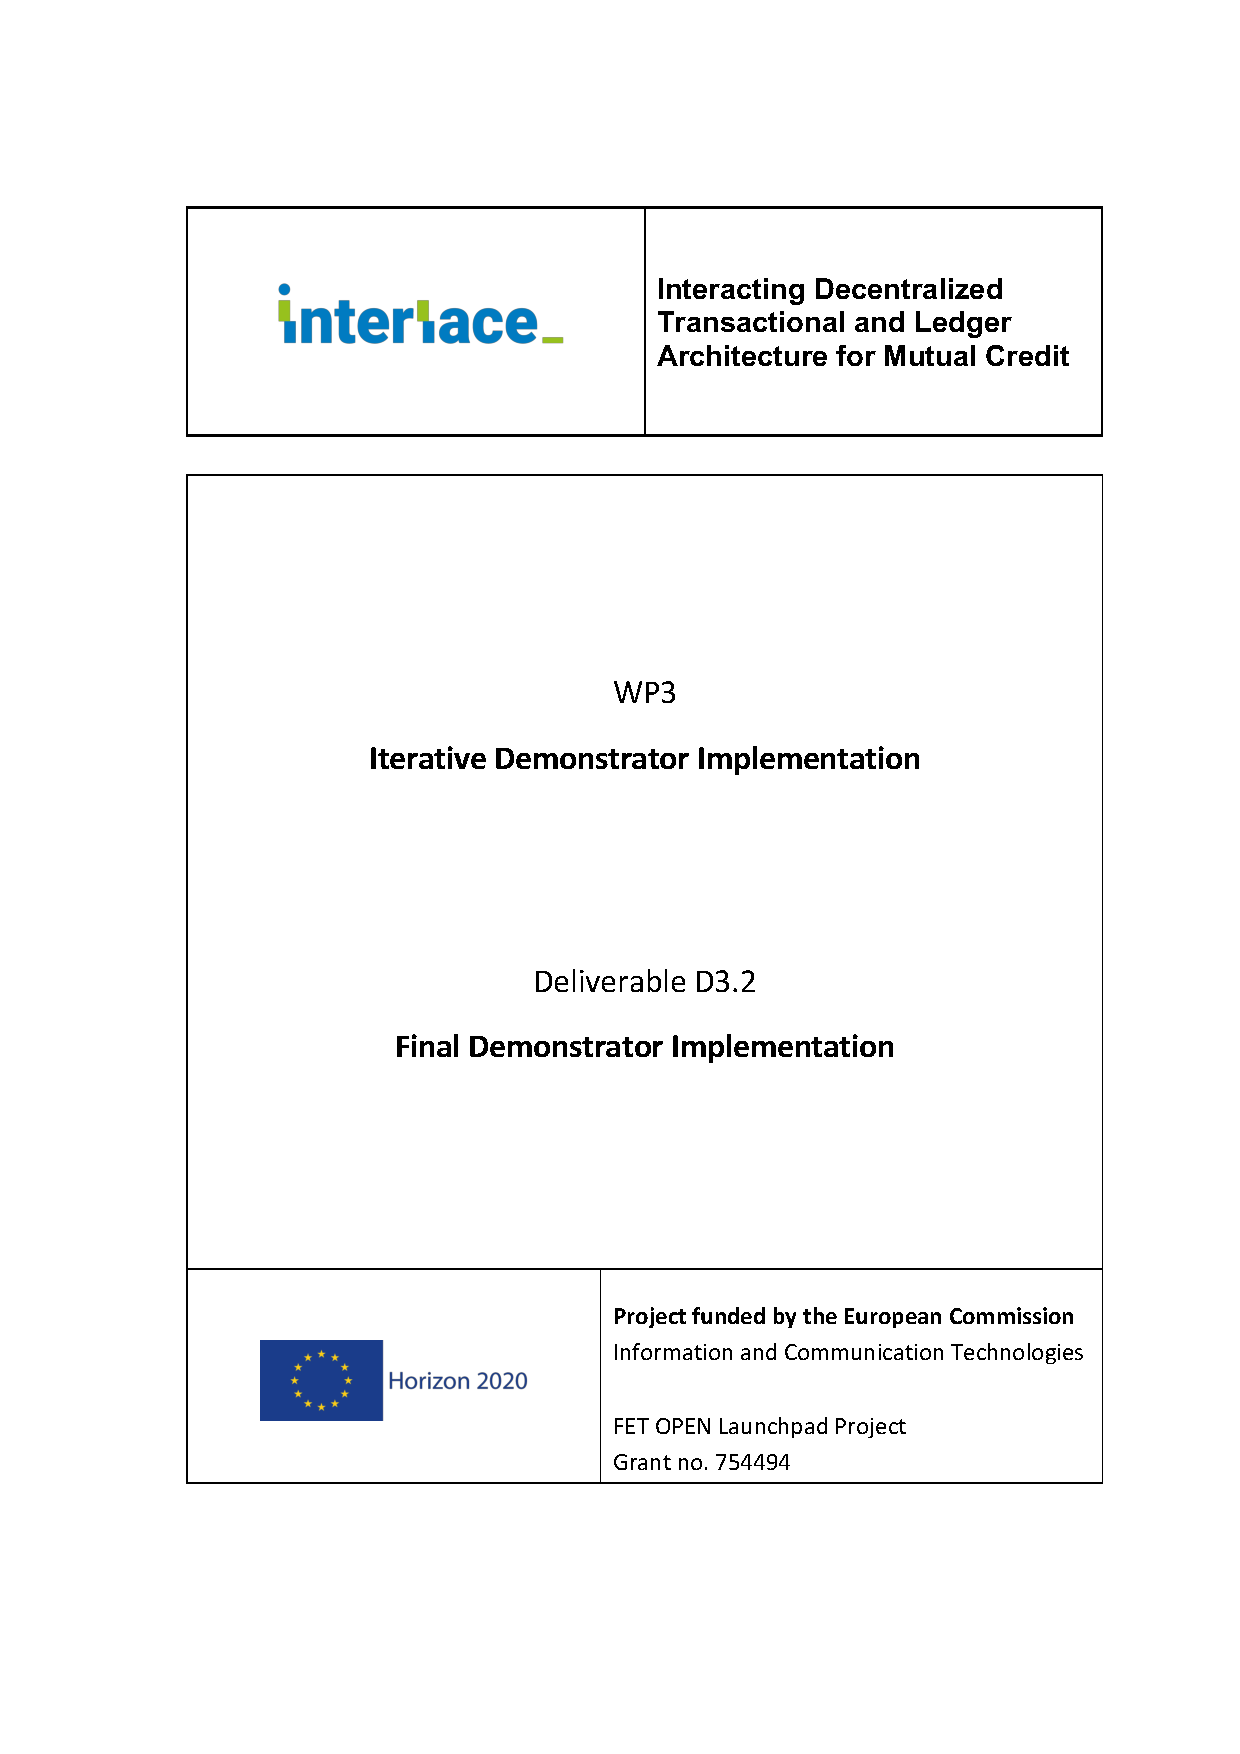
\includepdf[pages=-, scale=1.0]{Misc/Front}

%===================================================
%================== ABSTRACT
%===================================================
\thispagestyle{empty}

\begin{abstract}
\normalsize
This report describes the Hyperledger implementation of a part of the specification detailed in Delievarble D3.1: Requirements and Architecture Definition, as well as mechanisms used to ensure a stable and shared runtime environment and to guarantee testability and easy execution of the ASIM model of the business logic. The implementation is based on a refinement of the requirements that is detailed in this report, along with an updated formal specification, relative to the original ASIM definitions of D2.1, in the Appendix. Finally, a presentation of the runtime environment is given and discussed in the context of the future connection to the blockchain-based backend.
\end{abstract}

\newpage

%===================================================
%================== TABLE OF CONTENTS
%===================================================
\tableofcontents


%===================================================
%================== CHAPTERS
%===================================================
\chapter{Introduction}
\label{ch:Introduction}

\vspace{-1cm}
\begin{center}
Eduard Hirsch
\end{center}


\section{Objectives and Motivation}

During the INTERLACE project, requirements for the transactional platform of an interest-free mutual credit system were collected and documented in deliverables D2.1\cite{INTERLACE_D21} and D3.1\cite{INTERLACE_D31}. The requirements were formulated precisely using ``Abstracts State Interaction Machines" (ASIMs). These ASIM specifications were used to create a working ICEF implementation,\footnote{\url{http://biomicsproject.eu/news/135-icef.html}\\ \url{https://github.com/InterlaceProject/icef}} which also has been described in D3.1.

The focus of the present report is on the creation of a working prototype that provides basic payment capabilities, thereby enabling a scalable implementation of a distributed ledger technology (DLT).

\section{Scope and Organization}
This report provides insights into the prototype created. It discusses the technologies used and provides feedback on how they have been applied in order to achieve a working implementation capable of accepting basic transfers.

Further, information is given on how the system can be installed and used for paying. The system can therefore be used to prove and test various use cases in order to understand the chosen DLT approach.

For production systems, which might be built upon the INTERLACE prototype, important features are discussed that need to be handled during the realisation of such a payment system. Thus the transition from a client-server to a p2p-based model together with possible challenges are described and example approaches explained.

Finally, an outlook is given which elaborates possible scenarios that may be applied in a production context.

\newpage

%\input{2-}
%\input{3-}
\chapter{Conclusion and Final Thoughts}
\label{ch:conclusion}

\vspace{-1cm}
\begin{center}
Eduard Hirsch
\end{center}

This last chapter discusses the goals reached as well as the problems encountered during the development of the INTERLACE prototype. Additionally, it emphasises possible enhancements necessary and issues which need to be taken into account in order to bring the prototype to production level. Finally, it discusses parts that could not be finished as well as after-INTERLACE goals.

\section{Best Practices, Falsey Values and Pitfalls}

When using Hyperledger Composer but also when connecting to Hyperledger Fabric directly, it is important to pay attention to some points. Developers have to be aware that working with chaincode or smart contracts is quite different from accessing data as usual in a RDBMS,\footnote{Relational Database Management System} even though up-to-date frameworks shield a lot of the complexity underneath. Thus, even though access to the data structures and virtual machine/execution capabilities looks similar from a developer's point of view, it is necessary to account for some peculiarities related to blockchain-based technologies, because of their highly distributed nature. In the following sections we discuss and attempt to clarify some of these peculiarities.

\subsection{Deterministic Execution}

One of the most important things to keep in mind when writing chaincode applications is the deterministic execution of transactions. Although it seems quite obvious at first, it can be quite challenging to achieve.

One example is the \textbf{generation of IDs}: in a standard database environment simple locking mechanisms are in place to ensure correct primary keys for entries in a table. For blockchains which live in a distributed, consensus-based system it is problematic to create identifiers over chaincode execution. The reason is that each peer processing a transaction would compute a new ID completely independently, and most likely at the about the same time. Thus, if such a key-/ID-generation created different IDs on different clients, it might not be possible to reach consensus; thus, although nothing is actually wrong with the transaction itself, the resulting blockchain states in each peer would be different and therefore the last action would be rolled back. This would be especially hard to deal with during race conditions, and even more difficult to find out why a particular problem has occurred.

One solution to this problem could be to generate the ID from the client and pass it to the transaction as parameter. This would result in a much safer creation process which, additionally, is much faster during execution.

Another problem is posed by the use of \textbf{random numbers}. Since such calculations would reach different results on the various peers of the network,  creating random numbers in chaincode executions would cause sever problems when creating IDs from those numbers or randomizing decisions based on them, causing the results being indeterministic. Further, since it is not possible to know when a peer in the network will receive a new transaction, also the \textbf{creation of a date} or a timestamp contains an intrinsically random factor. Thus, dates created by different peer nodes during chaincode execution are prettly likely at least a bit different and when written into an e.g.\ asset are causing deviating blocks with different hashes of chains on the various nodes, and would therefore be rolled back when detected.

In listing \ref{lst:wrongDate} an example of a chaincode function is illustrated which creates a new date in line 8. The variable $currentDate$ will be filled with the current timestamp of the nodes Operating System.

\begin{center}
\begin{minipage}{0.8\textwidth}
\small
\begin{lstlisting}[language=javascript,firstnumber=1,caption={\bf\small An example of wrong determination of the current date inside of chain code}, captionpos=b,label=lst:wrongDate]
/**
 * CreditTransfer transaction
 * @param {net.sardex.interlace.CreditTransfer} transfer
 * @transaction
 */
async function CreditTransfer(transfer) {
  [...]
  let currentDate = new Date(); //incorrect!
  [...]
}
\end{lstlisting}
\end{minipage}
\end{center}

This implementation will lead as mentioned to inconsistent values of different peer nodes which may result in various problems.

For example, a possible scenario is that the date has been truncated to contain only day, month and year (no hour, seconds, ...), such that execution of the same transaction on different peers is likely to happen on the same day. In such a case, peers are able to reach consensus most of the time. However, validation of a transaction on different blockchain nodes would not be possible if it happens on different days (if e.g. execution is delayed or at the end of a day) or (re-)checked retroactively.

To explain further, chaincode running on peer $A$ may produce a date of 12 April 2018 at 23:59 in the evening. If peer node $B$ receives the same transaction at 00:00 the next day, it will produce the date 13 April 2018. Also, if e.g.\ somebody wants to check if the blockchain is in a consistent state, a transaction might be re-executed at any point in time after 12 April 2018 (staying with this example). Then the chaincode needs to run again and a date already written into the chain will be definitely different from the date produced during the re-execution. Consequently, those examples will lead to different outcomes on different peer nodes and therefore will trigger a rollback of the transaction or mark the whole chain as invalid from the point in time where that particular transaction had been appended to the ledger\footnote{Ledger structure: \url{https://hyperledger-fabric.readthedocs.io/en/release-1.3/ledger/ledger.html}}.

The solution to these kind of problems is to provide that possibly changing factor as an input parameter instead of creating it inside of the chaincode. Input parameters stay the same once a transaction proposal has been accepted and written into the chain. Thus, for every re-execution or validation they may be picked from there, allow re-run the code resulting in the same outcome every time when called. Therefore the re-generation of the the block hash will give the exact same hash like the "previous Hash" attribute of the the next block.

Given our Hyperledger Composer implementation the solution to the date problem could be to add an additional attribute for the abstract transaction $Transfer$ inside of our CTO-model definition, like adding $DateTime\ timeInitiated$. Then it would be necessary to pass a date value to the transaction for the $timeInitiated$ property when invoked by a client which then could be read from the transaction during chaincode processing.

However, in case of the date a better solution is offered by Hyperledger. When looking at the sequence diagram of the transaction flow\footnote{\url{https://hyperledger-fabric.readthedocs.io/en/release-1.3/arch-deep-dive.html\#swimlane}} which is prescribed by the Hyperledger protocol the very first step when proposing a transaction is to submit a $PROPOSE$ message to the endorsing peers which contain, beneath other things, the current timestamp which is further part of the transaction and finally stored into a block. Thus, the prototypical INTERLACE implementation is facilitating this timestamp to achieve the same goal like the propagation of the current date using the Transfer CTO-type. The code example in \ref{lst:correctDate} finally shows how the date may be read from the transaction.

\begin{center}
\begin{minipage}{0.8\textwidth}
\small
\begin{lstlisting}[language=javascript,firstnumber=1,caption={\bf\small An example of a correct determination of the current date inside of chain code}, captionpos=b,label=lst:correctDate]
/**
 * CreditTransfer transaction
 * @param {net.sardex.interlace.CreditTransfer} transfer
 * @transaction
 */
async function CreditTransfer(transfer) {
  [...]
  let currentDate = transfer.timestamp //correct!
  [...]
}
\end{lstlisting}
\end{minipage}
\end{center}


\textbf{Final note: Chaincode needs to be executed deterministically and has to reach, given its input parameters, the same result(s) on all the peer nodes at any point in time}. Consequently many parameters cannot be generated by chaincode directly but need to be provided as parameters to a transaction. But since this means that the parameters are creatable on the client-side only, it is also necessary to implement the corresponding logic in a way that prevents them from being used to fool the system or bring it into an inconsistent state.

\subsection{Network Upgrade}

Traditionally, updating a database after changes to the database model may be quite cumbersome due to the presence of new fields, foreign keys, and many other similar issues. However, various methods and strategies are in place for handling these issues.
On the other hand, since blockchains are usually spread over various peers that store replicated data, in contrast to traditional databases it is inherently more difficult to change the distributed structures to fit some new schema necessary to add a new feature or functionality.

Updating or changing values of asset attributes, as well as getting executable code and data structures ready for the next version of the network, may run into several problems. In particular, in order to maintain consistency and reliably achieve all fixes it is necessary to apply all changes to the network in such a way that upgrading the business network (CTO-File, chaincode, ...) and fixing the asset values happen in the right order, and while nobody else is able to interfere. This can be achieved by executing the upgrade as a single atomic transaction or, if that's not possible, by blocking common user access during deployment.

Thus, it is quite important to get everything right from the beginning, as it can be extremely difficult to apply certain changes. Consequently, it is highly advisable to think about possible changes and future scenarios together with possible side-effects and costs before first deployment to production systems.

\subsection{Hyperledger Composer Specifics}

Composer can be seen as a rapid-development approach. Its API sits on top of the Hyperledger Fabric framework. It tries to shield complexity from the user and aims to significantly reduce the time necessary to create distributed applications for Hyperledger Fabric.

For the development of the INTERLACE transactional service this meant that:
\begin{quote}
\vspace{-0.3cm}
\begin{itemize}
	\item models could be transferred easily,
	\item chaincode could be based on these models,
	\item a REST Server was supplied and
	\item a web-application generator was available.
\end{itemize}
\vspace{-0.3cm}
\end{quote}
Consequently, it was an ideal framework for prototyping. In addition, once a suitable cloud provider has been found, spinning up a network is straightforward. When hosting a network without an external provider who knows how to run these networks, much of the initial speed in creating it might be lost because, in such a case, a much deeper understanding of the whole architecture is necessary. Thus, also a greater effort is needed to get a ready implementation to work.

\textbf{Note:} For production systems it would be necessary to change to a plain Fabric implementation because Composer is still at quite an early stage of development, and there are even rumours that it may be discontinued. The reason is that some of the new features of the Fabric releases are deviating from the structures implemented by Composer. So it is becoming increasingly difficult for Hyperledger Composer developers to provide new features and functionalities available for Fabric.

\section{Identity Management}
\label{sec:id-management}

As mentioned in previous sections, we skipped Identity Management for the prototype in order to simplify the environment, decrease development efforts and therefore offer a relatively easier access to an example mutual credit system, hoping that this would make it easier to understand the basics. Nevertheless, it would be possible and quick to create additional participants and grant them access to the network in addition to just the currently used admin account. For example, an identity card can be issued for the first participant defined in transaction "InitBlockchain" which is identified by "m1". The example below illustrates how this might be done:

\begin{lstlisting}[language=bash]
	composer identity issue -c admin@tutorial-network -f m1.card -u m1 -a "resource:net.sardex.interlace.Individual#m1" -x true 
\end{lstlisting}
\vspace{-0.3cm}

This identity card is facilitated by the REST server and corresponds to a participant in the business network. 
But, when accessing the REST server, before a user can act with that identity it is necessary for him/her to log in first and authenticate his/her identity in some sort of way. To do so composer-rest-server uses an authentication middleware implemented in JavaScript called \textit{Passport.js}.\footnote{\url{http://www.passportjs.org/}}

The passport middleware offers many different authentication strategies and is quite a mature Open Source framework. An example of how to authenticate with OAuth and GitHub can be found on the Composer documentation website;\footnote{\url{https://hyperledger.github.io/composer/latest/integrating/enabling-rest-authentication}} but also different schemes can be used, like the JSON Web Tokens (JWT\footnote{\url{https://jwt.io/}}) which is mentioned in the issue tracker of the Hyperledger Composer GitHub page.\footnote{\url{https://github.com/hyperledger/composer/issues/2038}}

Passport is a commonly known middleware for authentication and may be applied also to different scenarios. Thus, it is usable well also if Composer is swapped for another technology.

\section{Future Scenarios}
\label{sec:future-scene}

Because we are using Hyperledger Fabric, extending the network is only a matter of changing the configuration. The approach taken for the INTERLACE prototype, shown in Figure \ref{fig:prototype-net-ext}, creates a new organisation for every payment circuit that deals with a new specific region. Consequently, each region would be responsible for hosting their own peers and ideally also their own certification authority (CA). However, certificates might be still handled by the Sardex CA. 

Sardex, in this scenario, is providing the network architecture and transferring the know-how about how to run a circuit, which would result in a model similar to a franchise. Although the clients and various other visible graphical interfaces may be branded in various ways, the underlying platform infrastructure would be predefined by Sardex in order to make the network work consistently.

The orderer will be handled by Sardex as well, but later might be handed over to an e.g.\ non-profit organisation representing the circuit and enforcing fair and clearly defined rules within a governance framework defined in collaboration with the circuit members themselves. To ensure a reliable system and a high performance throughput, an orderer could be clustered locally but also over various regionally separated areas.

\begin{figure}[htbp]
  \centering
  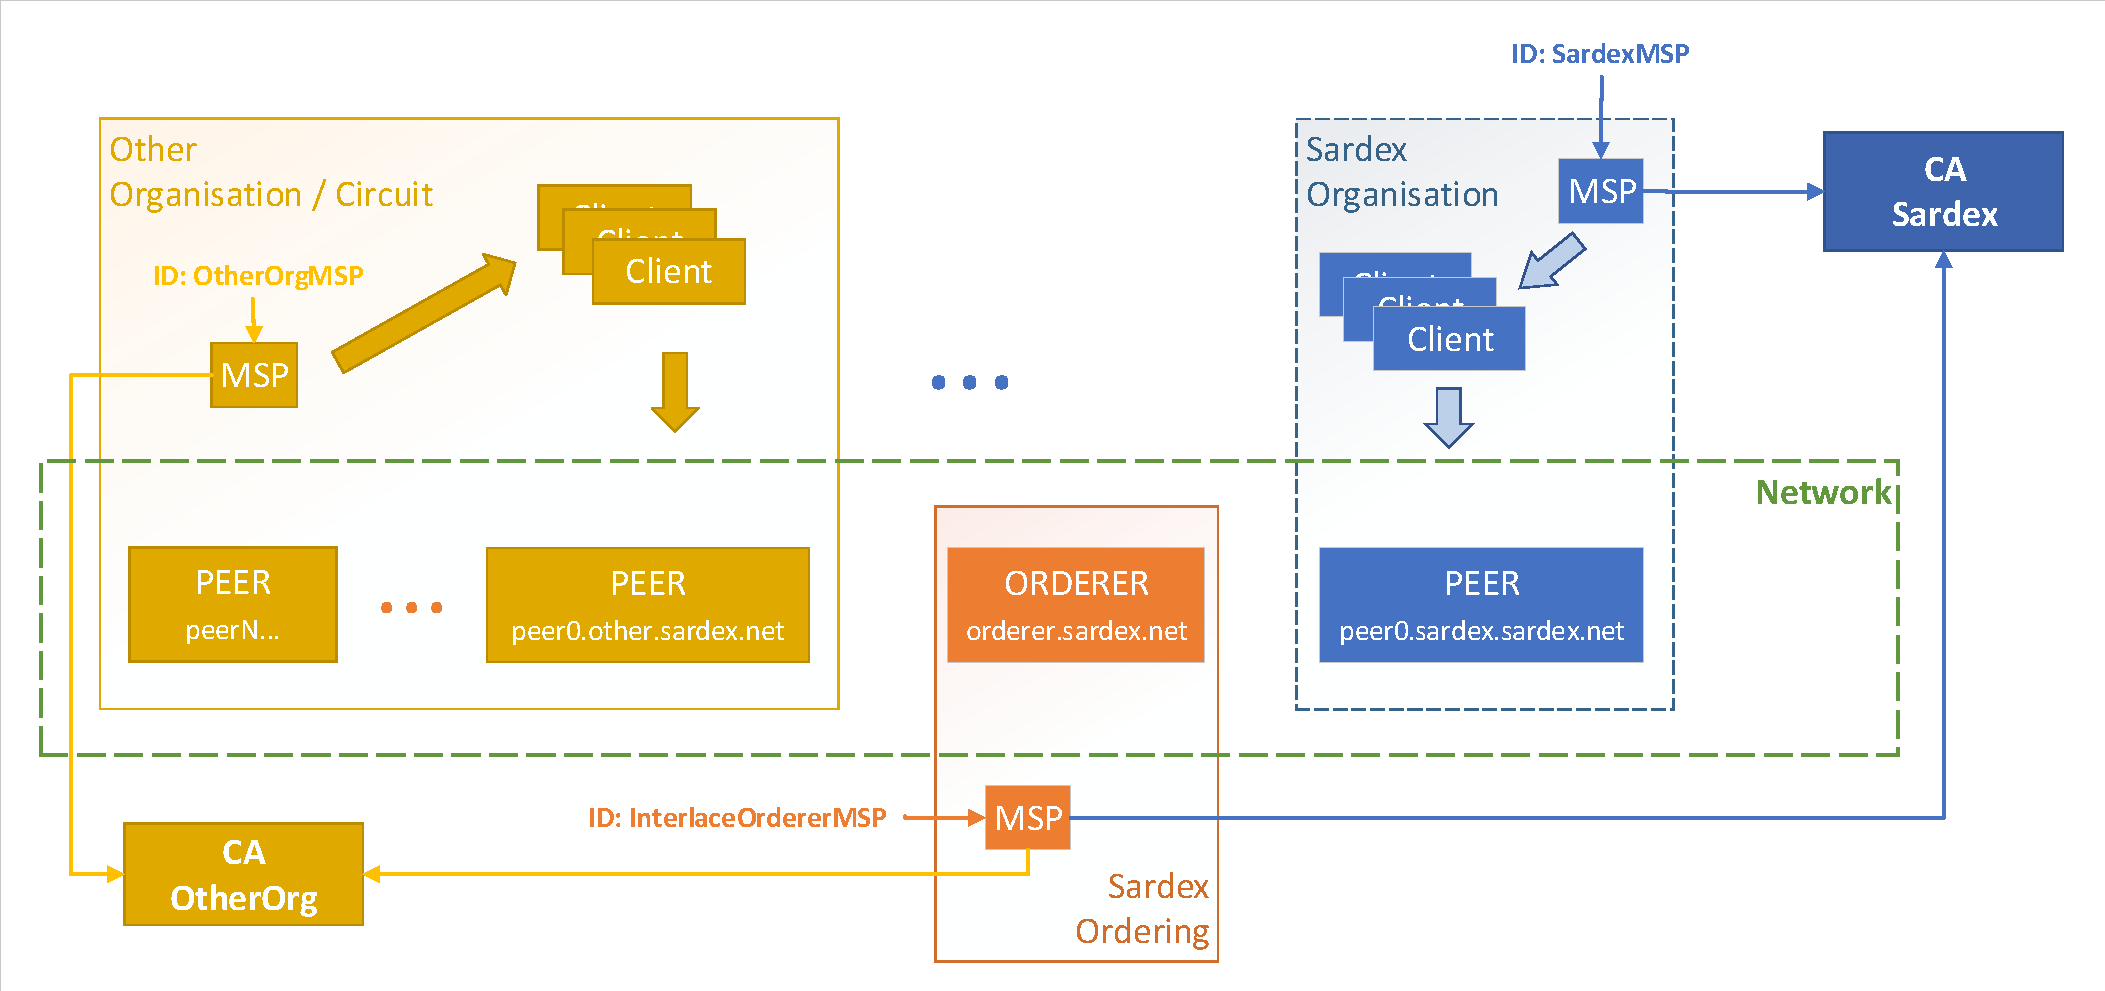
\includegraphics[width=1.0\textwidth, clip, trim=1mm 1mm 1mm 1mm]{Figures/extended-network}
  \caption{\bf\small Extended Network Structure}
  \label{fig:prototype-net-ext}
\end{figure}

\section{Final Review and Open Points}

Our DLT application prototype forms a stable and scalable basis for a reliable payment circuit. In fact, although the prototype was developed with Hyperledger Composer, which IBM may discontinue support for, any subsequent implementation in Hyperledger Fabric only will now be much easier to realize. This is also because newer versions of Fabric support a node.js SDK,\footnote{Software Development Kit} which would even allow the transfer of JavaScript code bits.

In summary, the goal of creating a reliable DLT has been achieved, and forms a necessary foundation for the various other services provided in future for the production-level business solutions created by and with Sardex.

\subsection{Open Points}

The \textbf{GDPR}\footnote{General Data Protection Regulation \cite{GDPR}} directive that came into effect in the first half of 2018 represents a challenge for blockchain solutions and, therefore, also for the INTERLACE project. It is necessary that personal information is not exposed to other parties unless necessary and unless it is done in agreement with its owners. In addition, each piece of information collected for the user or provided by the user needs to be deletable if the user requests it, and it must certainly be possible to look up upon request exactly what data was collected.

Information is reliably stored inside of a blockchain. Thus, looking up information is actually not an issue. Rather, one of the challenges is to keep it secret from being read by other parties, since standard blockchain approaches copy everything to every peer. Another challenge is the immutability of most blockchains, since GDPR enforces the right to be forgotten. The privacy aspect is solved currently by making the actual chain only accessible by the peers that are owned by the organisation running the local circuit. In this configuration, the clients that perform transfers have restricted access and cannot see the whole blockchain.

In later stages it may be possible for every business/party participating in the payment network to access the blockchain directly, i.e.\ to run a node. In this case the so-called \textit{SideDB}\footnote{\url{https://hyperledger-fabric.readthedocs.io/en/latest/private-data/private-data.html}} can be taken into consideration because it is a way offered by Hyperledger Fabric to store information which is only known by the respective client and only shared if permitted by the client.

\textit{SideDB} also solves the problem of GDPR-relevant data because, first, it is only exposed ``to whom it may concern'' and, second, it can be purged without making the chain invalid. The reason is that in SideDB only hashes of transactions and data are stored on the chain, which still makes it verifiable by regenerating the hash and comparing every time a datum needs to be verified. Normally the data only needs to be provided if specifically asked for, e.g.\ in case of an (external) audit.

The second point which needs further effort is the part of the testing coverage where the \textbf{ASIM implementations} are \textbf{tested} against the actual implementation of the prototype and later against the production-level implementation. These tests will be covered in deliverables D4.1 and D4.2 whose future versions will be completed after the end of the project.








%\input{2-DLTs_Selected/dlt}
%\input{3-Functional_Requirements/funreq}
\chapter*{References}
%\renewcommand{\section}[2]{}

\setlength{\parskip}{0.8\baselineskip}
\bibliographystyle{plainurl}
{\small
\addcontentsline{toc}{chapter}{References}
\bibliography{Bib/BioComp_References}}


%===================================================
%================== APPENDIX (1st way, used in D3.1)
%===================================================
%\appendix
%\addcontentsline{toc}{chapter}{Appendix: Complete Functional Requirements and Business Logic Model (2018)}
%\setcounter{chapter}{1}
%\renewcommand\thechapter{}
%\makeatletter
%\renewcommand\thesection{\@Alph\c@chapter.\@arabic\c@section}
%\makeatother
%\input{6-Appendix/SardexNewPaymentSpec_V6}


%===================================================
%================== APPENDIX (2nd way)
%===================================================
%\begin{appendix}
%\section*{Appendix}
%\includepdf[pages={-}]{sections/4-CaSM/CaCycleAsm.pdf}
%\end{appendix}

\end{document}
